\newcommand{\h}{$h(\vec x)$}
\newcommand{\e}{\epsilon}
\chapter{Neural networks}\label{chapter:symmetries}

\section{Introduction into artificial neural networks}

\section{The ROC curve and the optimal classifier}
One of the most common problem in machine learning is a binary classification, when a data set has to be divided into two subsets, fulfiling serian requirements. A simple example of such a problem is distinction between signal and bacground events in deta collected by experiment. We would like to have a function which takes as agruments set of physical observables (eg. particles' energy, momentum, coordinates of vertexes), represents by $\vec{x}$ and returns sigle number. More formally, a clasyfier can be call any function $h: \vec x \rightarrow \mathbb{R}$ designed in such a way, that high \h values correspond signal events and low \h values correspond background event. A threshold value  \h =c, which is the value separating signal and backgrond events is called a working point, and has to be set by a user. The signal efficiency will be defined as $\e_S=\int d\vec x \rho_S(\vec x) \Theta(h(\vec x) -c)$ and respectively a background efficiency $\e_B=\int d\vec x \rho_B(\vec x) \Theta(h(\vec x) -c)$.

The problems how to represent a clasyfier performence, how to compare different clasyfiers and how to choose proper working point have been discused since many years. 

\section{The data-driven approach}
The original paper by Metodiev, Nachman and Thaler \cite{Metodiev_2017} the othors show the idea of a data-driven analysis in details. In this chapter I want to introduce main concepts, necessery to understand how the proposed metode helps in week decays recosntruction.

In a classical approach to supervized machine learning, a model learns its properties usign sets of labeled data. Of courese providing good training sets is always a problem. To do this someone can use either experimental data, labeled by a user, or simulation. In first case a user uses his external knowledge about the data to describe it. In necond case the user fully rely on simulation. (opisz zagrożenia)

The data-data driven analysis avoids inconveniencees of two mentioned methodes. It requires neither labeling nor simulation. According to Neyman-Pearson lemma \cite{Neyman-Pearson} the optimal clasyfier for two sets, A and B is a function given by a dencity ratio
\begin{equation}
  \label{eq:N-P}
  h_{opt}^{A/B}(\vec x)=\frac{\rho_A}{\rho_B}
\end{equation}
or any monotonous function of $\frac{\rho_A}{\rho_B}$. Assuming that both sets A and B contains signal (s) and bacground (b) events and a statistical distribution of s and b is the same in A and B, we can write \eqref{eq:N-P} in the following way
\begin{equation}
  h^{A/B}_{opt}=\frac{f_1 \rho_s + (1-f_1) \rho_b}{f_2 \rho_s + (1-f_2) \rho_b}=\frac{f_1 \rho_s/\rho_b+1-f_1}{f_2 \rho_s/\rho_b+1-f_2}=\frac{f_1 h_{opt}^{s/b}+1-f_1}{f_2 h_{opt}^{s/b} +1-f_2}.
\end{equation}
It can be proven that $\partial_{h_{opt}^{s/b}}h_{opt}^{A/B} >0$, what means that optimal clasyfier for both cases is the same. It is important to underline that the reasoning gives no clue about the working points for both cases.

\begin{figure}[ht]
  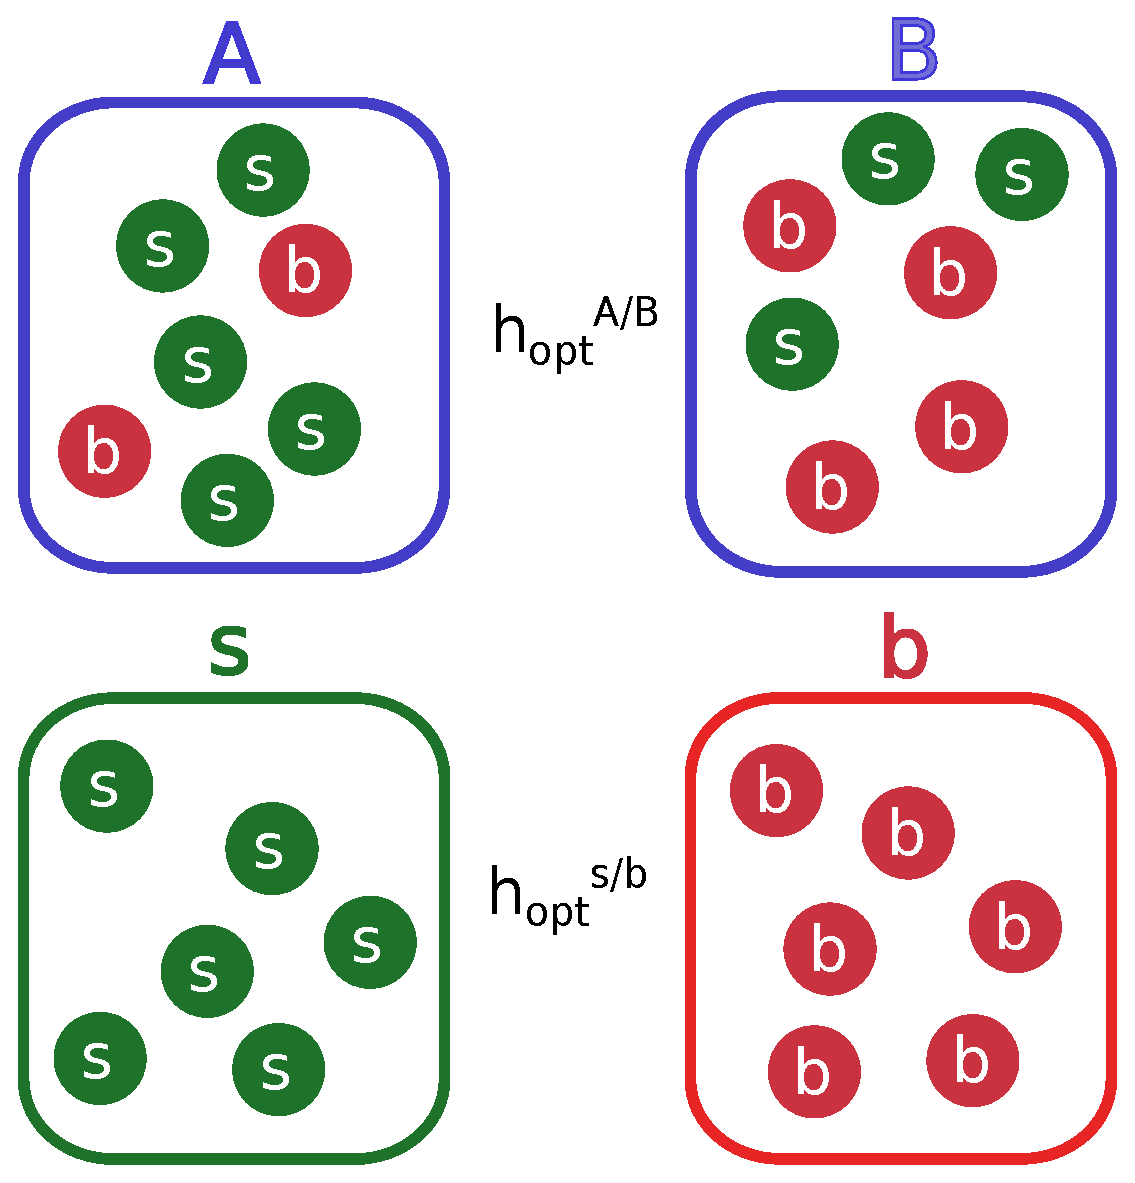
\includegraphics[width=0.5 \textwidth]{Chapter_NN/setAB.eps}
\caption{A data-driven approach visualisation. According to \cite{Metodiev_2017} the opitimal clasyfier for sets A and B is equivalent to optimal clasyfier for sets s and b.}
\end{figure}

\section{Application for analysis}
In case of $\Ls$ reconstruction the data driven approach was used to replace set of geometrical cuts and enchace a $\Lz$ signal, so for the neural network all events with $\Lz$ were treated as a signal and without like a background. For all events an invariant mas of $\p \pim$ pair was ploted. Using this spectrun I have divided the dataset in two subsets: for $M^{inv}_{\p\pim} \in (1015,1125)$ and $M^{inv}_{\p\pim} \notin (1015,1125)$. In the first of them a ratio between $\Lz$ and background is clearly different than in the secon.    


%%% Local Variables:
%%% TeX-master: "../main"
%%% End: 